
\documentclass[a4paper]{article}
\usepackage[french]{babel}
\usepackage[utf8]{inputenc}
\usepackage[T1]{fontenc}
\usepackage{amsfonts,amsmath,amssymb}
\usepackage{graphicx}

\title{Examen - Fondamentaux théoriques en Machine Learning}

\author{Nicolas Bourgeois}

\date{SCIA, S9, 2020-2021}

\begin{document}

\maketitle

\textit{L'examen dure 2 heures. Tous les documents sont autorisés. Le rendu s'effectue au format pdf dans un seul fichier \textbf{dont le titre doit inclure votre NOM et votre PRENOM} Les graphiques peuvent être réalisés avec n'importe quel logiciel/librairie ou même scannés. Les exercices sont indépendants.}\\

\textbf{Exercice 1}\\

a) Produisez les matrices de confusion respectives associées aux deux estimateurs figurés par les droites suivantes (NB : il y a 50 points dans chaque classe, les triangles correspondent à Y=1, les ronds à Y=-1)\\

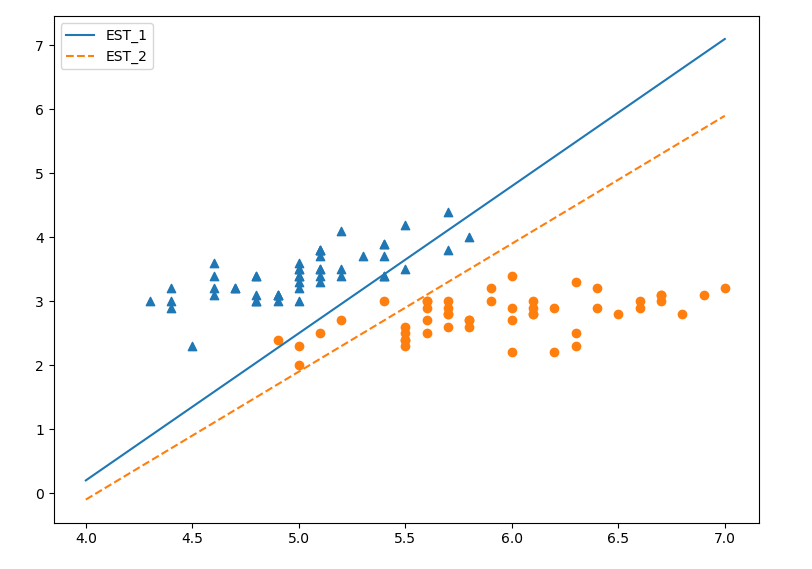
\includegraphics[scale=1]{estimateurs}

b) On considère la fonction de perte asymétrique suivante :\\

$ y0 > y \Rightarrow LF(y; y0) = 1.5$ ; $y0 < y \Rightarrow LF(y; y0) = 0.9 $\\

Calculez l'ERM des deux estimateurs.\\

c) Supposez que EST\_1 soit un SVM. Que peut-on affirmer à coup sûr concernant son coefficient de pénalisation ?\\

\textbf{Exercice 2}\\

A partir des tableaux de données ci-dessous, produisez l'estimateur bayesien naïf associé à l'obervation X = (FALSE, TRUE, FALSE).\\

\begin{tabular}{|l|l|l|}
\hline
Y=True & X=True & X=False\\
\hline
X1 & 13 & 43\\
X2 & 32 & 24\\
X3 & 7 & 49\\
\hline
\end{tabular}

\vspace{0.3cm}

\begin{tabular}{|l|l|l|}
\hline
Y=False & X=True & X=False\\
\hline
X1 & 1 & 24\\
X2 & 15 & 10\\
X3 & 14 & 11\\
\hline
\end{tabular}

\vspace{0.3cm}

\textbf{Exercice 3}\\

Prouvez que la dimension de Vapnik-Chervonenkis du preceptron monocouche sur les sommets d'une pyramide à base carrée est exactement 4.\\

\textbf{Exercice 4}\\
A partir du tableau de données ci-dessous, produisez un arbre de décision de profondeur 2 de risque minimal.\\

\begin{tabular}{|l|l|l|l|}
\hline
X1 & X2 & X3 & Y\\
\hline
T &F &T &F\\
T &F &F &F\\
T &T &T &T\\
T &T &F &F\\
F &T &T &T\\
F &T &F &F\\
F &F &T &T\\
F &F &F &T\\
\hline
\end{tabular}

%%%%%%%%%%%%%%%%




\end{document}
